\documentclass[12pt, a4paper,oneside]{report}
\usepackage{titlesec}
\usepackage[utf8]{inputenc}
\usepackage{german}
\usepackage[T1]{fontenc}
\usepackage{textcomp}
\usepackage{framed}
\usepackage{pbox}
\usepackage{caption}
\usepackage[nottoc,numbib]{tocbibind}
\usepackage[pdftex]{graphicx}
\usepackage[toc]{glossaries}
\usepackage{amssymb, amsmath}
\usepackage[colorlinks,
pdfstartview = FitH,
linkcolor = black,
plainpages = false,
hypertexnames = false,
citecolor = black]{hyperref}
\usepackage{setspace}
\onehalfspacing
\usepackage[left=3.5cm,right=3.5cm,top=2cm,bottom=2cm]{geometry}
\graphicspath{{./pics/}}
\usepackage[printonlyused]{acronym}
\usepackage{todonotes}
\usepackage{subcaption}
\usepackage{float}
\usepackage{pifont}
\newcommand{\cmark}{\ding{51}}%
\newcommand{\xmark}{\ding{55}}%
\usepackage{multirow}
\usepackage{pdflscape}
\usepackage{eurosym}
\usepackage{tocbibind}
\usepackage[english]{babel}
\usepackage[utf8]{inputenc}
\usepackage{multirow}
\usepackage{subcaption}
\usepackage[section]{placeins}
\usepackage{lscape}
\begin{document}

\begin{titlepage}
	Universität Passau\newline
	Fakultät für Informatik und Mathematik
	\vspace{2.5cm}
    \begin{center}
    \LARGE\textbf{{Classification  Of Visualization  In Scientific Literature}}\\
   
    \normalsize

    \vspace{2.5cm}
    \end{center}

 \normalsize{
 	Masterarbeit zur Erlangung des akademischen Grades\newline
 	Master of Science (M.Sc.)\newline
 	\ \\
 	Lehrstuhl für Intelligent Systems und Lehrstuhl für Data Science \newline
 	der Fakultät für Informatik und Mathematik\newline
 	der Universität Passau\newline
 	
 
    \begin{tabular}{ll}
    	Name: & Arnold Azeem \\
    	Matrikelnummer: & 79176 \\
    	Fachbereich: & Informatik\\
    	Studiengang: & Master Informatik\\
	Erstprüfer: & Prof. Dr. Christin Siefert \\
	Zweitprüfer: & Prof. Dr. Michael Granitzer\\
	Date: &     \today
    \end{tabular}\\
    }



\newpage
\begin{abstract}
Distinct visualisation techniques are used in scientific research publications to summarise large amount of data and also represent a variety of data. These visualisations help to communicate complex information and support the arguments being presented in the publication in a way that is easy to understand and follow.
These figures tend to reveal trends, patterns or relations that might have otherwise been difficult to grasp using only text. 
It is therefore relevant that we extract the data from these visualisations since the extracted data can be used for validating the publication or presenting the data in another form for a different audience. In this context, classifying these visualisations is the initial step since, there is a variety of visualisations and each one is processed in a specific way. It is only after classification that extraction of raw data from these visualisations can be acquired for other tasks. This thesis presents an approach whereby real world data is used to create four types of plots (scatter plots, bar charts, line charts, and box-plots) and random plots also of the same kind from the Internet are added together and used to train and evaluate a CovNet model to be able to classify these plots. 
\end{abstract}

\renewcommand{\abstractname}{Acknowledgements}

\end{titlepage}

\setcounter{tocdepth}{10}
\tableofcontents


% \begin{acronym}

% \acro{XML} {Extensible Markup Language}s

% \end{acronym}

\listoffigures
\listoftables

\titleformat{\chapter}{\LARGE\bfseries}{\thechapter}{1em}{}

\newpage
\chapter{ABSTRACT}
Distinct visualization techniques are used in scientific research publications to summarize large amount of data and also represent a variety of data. These visualizations help to communicate complex information and support the arguments presented in the paper in a easy to understand and follow way.
These figures tend to reveal trends,patterns or relations that might otherwise be difficult to grasp using only text. In this context, classifying these visualizations is really relevant since there is a variety of visualizations and each one will have a different approach to processing it, example is extracting the raw data from it. 

\chapter{INTRODUCTION}
A picture tells a thousand words even though a cliché stands to be very true especially when it comes to presenting complex findings in scientific research publications. The importance of these figures in papers cannot be undermined since they provide a way to easily interpret,find patterns and relations in the data which would have otherwise been more complex relying on  only textual data. All though extracting data from a plot manually is relatively easier, doing the same task automatically requires each type of plot to be processed specifically. In this work we present a way to classify each plot effectively, since that the first step before further processing of a plot is possible.  


\section{MOTIVATION}
Complex data is better explained in scientific papers with the aid of visualizations. These plots present complex data in an easy to understand way compared to textual representation. The data which these visualizations contain when extracted play an important role in events where another researcher wants to verify the work of the publisher, this data can also be used to develop other visualizations in situations where the paper needs to be presented to a different audience with a different background as opposed to the audience which the visualizations were created for, Also when comparing two plots the raw data helps make a better decision than just the figures. Since each plot will be processed differently to extract the raw data, it very relevant that we can distinguish one plot from another and this is the main aim of this thesis. 

\section{OBJECTIVE}
The purpose of this thesis is to answer the question: \begin{quote} HOW WELL CAN WE CLASSIFY THE DIFFERENT TYPES OF PLOTS IN SCIENTIFIC LITERATURE.\end{quote} In this work we focus on only four plots. These plots are scatter plots,bar charts,line charts and Box plots. The diagram below shows the vision of this work, The first part of the diagram involves extracting or obtaining  the four different types of plots mentioned earlier,after which we then label our plots and train a neural network model to be able to classify with high accuracy any of the four plots if shown to our model, then finally the raw data can be extracted from the detected plot.
But this work mainly focuses on the red dotted lines shown below in the diagram which which is getting the plots, labeling them, training the model and classifying the plots. \\
 
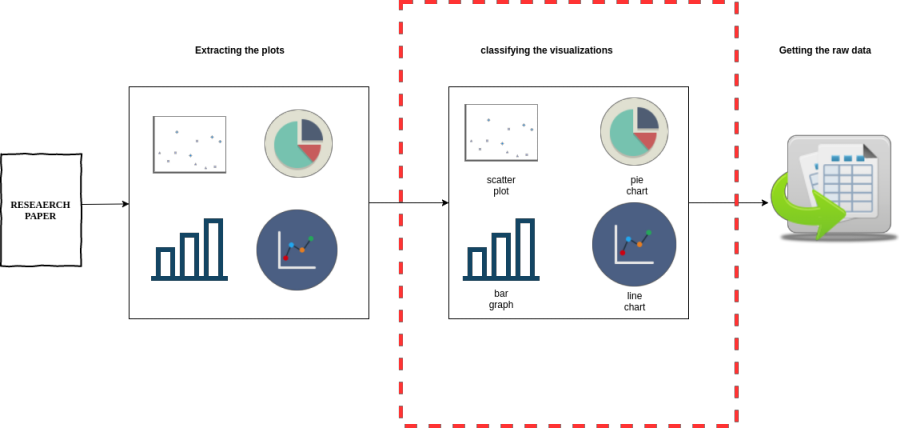
\includegraphics [scale=0.5] {vision}
\captionof{figure}{vison of the thesis}

\chapter{RELATED WORK}
Our work is inspired by Architecture proposal for data extraction of chart images using Convolutional Neural Network(2017) \cite{junior2017architecture}, In this paper, they propose a way to gain the wealth of information contained in different visualization techniques. The paper talks about two main stages of accomplishing this task. Firstly, classification of the charts is done since it allows a different variety of chart to be detected automatically allowing the next step, which is the extraction of data from the classified plots. The paper, however, focuses on the first step, classification of charts. In this paper, a Convolutional Neural Network is used for the classification task. The Convolutional neural network encapsulates the characterization and classification processes during its learning process, unlike other techniques. The dataset used for this task were searched for and downloaded from Google image search. Table \ref{table:rela} shows the chart types which were collected and the number of train and test sets which the respective charts were divided into.

\begin{table}[h]
	\centering \def\arraystretch{1.5} \small
	\begin{tabular}{|p{5cm}|p{3cm}|p{3cm}|}
		
		\hline
		Chart Type & Test & Train \\ \hline
		Area Chart & 50 & 555 \\ \hline
		Bar Chart & 50 & 657 \\ \hline
		Line Chart & 50 & 489 \\ \hline
		Map & 50 & 476 \\ \hline
		Pareto Chart & 50 & 261 \\ \hline	
		Pie Chart & 50 & 361 \\ \hline
		Radar Chart & 50 & 454 \\ \hline
		Scatter Chart & 50 & 552 \\ \hline
		Table & 44 & 236 \\ \hline
		Venn Diagram & 48 & 304 \\ \hline
		Total & 498 & 4345 \\ \hline
		
	\end{tabular}
	\caption {Number of Train and Test Dataset collected}	
	\label{table:rela}
	
\end{table}
For the classification, a variant of convolutional neural network called LeNet-based CNN model is used. The model was implemented using \footnote{Tensorflow}, LeNet-based CNN has an architecture which is comprised of 3 convolutional layers, followed by a fully connected layer. The model is trained in a way that the dataset is divided into mini-batches, samples of fixed sizes(100) are selected and fed into the CNN, as a result of this process the model becomes robust since it learns to generalize from the different min-batches which are fed into the model. Also, all the images are converted to JPG and resized to 224x224x3, that is, 224 pixels of height, 224 of width and 3 layers of output. The other parameters used were 1000 epochs and a learning rate of 0.003. The accuracy at the end of the training process was 70\%.


\section{Dataset}
In this section, the various datasets used in plotting are described. For each language a different set of CSV files are used for generating the plots. This is done to generate more diverse plots.

\subsection{Dataset for Matlab}
The Data used for creating the plots in Matlab were randomly chosen from Project Dataset \cite{projectdataset}, a free CSV data repository, DatPlot \cite{datplot} and Plotly CSV repository in github \cite{plotly}. The datasets are multidimensional and compiled from normal day to day activities like dating, what makes people happy etc, and objects like cameras and cars. On the average the datasets used contain about 500 instance and 5 different columns. The biggest dataset is called Speed dating data. It is made up of over 8,000 observations of answers to survey questions about how people rate themselves and how they rate others on several dimensions. The smallest dataset used has 33 instances and 12 columns. It contains information about cars. The number of gears and speed, just to name a few attributes.

\subsection{Dataset for R}
For the plots in R, 13 random CSV files where downloaded from an archive of datasets distributed with R called Rdatasets  \cite{rdata}. Rdatasets is a collection of dataset distributed with R. On the average there are 80 instances and 5 columns in each dataset.
The biggest CSV file is the Australian athletes dataset. Its made of 203 instances and 14 columns and contains attributes like sex,height,weight and sports. The smallest dataset is the Canadian Women's Labour-Force Participation. This dataset has 30 rows and 7 columns. It contains information like average wages of women, percent of adult women in the workforce etc.


\subsection{Dataset for PYTHON}
The data used for creating the plots in Python were 15 randomly seleted csv files also from  Rdatasets \cite{rdata}. The biggest dataset among the 15 is the Monoclonal gammapothy data, it contains natural history patients with monoclonal gammapothy of undetermined significance. The dataset is made up of 1384 observations with 10 columns, it has attributes like age, sex, time of death and last contact in months. On the average each dataset contains about 200 instances and 7 columns of multi-dimensional data. The smallest dataset however contains only 33 instances with 11 columns and is called the Nuclear Power Station Construction Data.The data relate to the construction of 32 light water reactor (LWR) plants constructed in the U.S.A in the late 1960's and early 1970's.

\subsection{Dataset for Java}
For the plots created in java, I used the dataset made available by Plotly \cite{plotly}, a github repository of CSV datasets used in the Plotly API examples. 14 random CSV files were downloaded, the biggest file has 1002 instances and 9 columns, and on the average each file contains about 100 instances and 9 columns. The smallest file however is made of 33 instances and 12 columns called the mtcars file. It contain information about a variety of different car models like the number of gears, speed etc. The table \ref{table:1} contains the names of all CSV files that were used in the different languages with the different plotting programs.


\begin{table}[h]
	\centering \def\arraystretch{1.5} \small
	\begin{tabular}{|p{5cm}|p{3cm}|p{3cm}|p{4cm}|}
		
		 \hline
		 \multicolumn{4}{|c|}{DUMMY DATA} \\
		 \hline
				
		PYTHON & MATLAB & R LANGUAGE & JAVA\\ \hline
		
		3d\_line\_sample\_data.csv \par LightFordwardFlapStall.csv  \par line\_3d\_dataset.csv \par
		longley.csv  \par loti.csv  \par lung.csv  \par nuclear.csv  \par timeseries.csv  \par
		USJudgeRatings	\par WVSCulturalMap.csv  \par wind\_rose.csv  \par volcano.csv  \par uspop2.csvm &
		
		Camera.csv \par Cars.csv \par CausesOfDeath-France.csv \par Cereal.csv  \par happiness.csv \par TestData1.csv \par TestData2.csv  \par mpg.csv \par okcupid-religion.csv  \par spectral.csv
		\par stockdata.csv \par subplots.csv  & 
		
		ais.csv \par Angell.csv  \par Baumann.csv \par Bfox.csv \par cane.csv \par carprice.csv \par Chirot.csv
		Davis.csv \par Ericksen.csv \par Florida.csv \par Highway1.csv \par Pottery.csv \par Prestige.csv 
		salinity.csv \par urine.csv & 
		
		3d-line-plot.csv \par 3d-scatter.csv \par 2011\_flight\_paths.csv \par 2011\_us\_exports.csv \par auto-mpg.csv \par candlestick\_dataset.csv \par finance-charts-apple.csv \par 
		globe\_contours.csv\par hobbs-pearson-trials.csv \par motor\_trend\_tests.csv \par 
		nz\_weather.csv \par volcano.csv \par iris.csv \par mtcars.csv	\\ \hline
		
	\end{tabular}
	\caption {Names of CSV files used in each language}	
	\label{table:1}
\end{table}


\chapter{CREATING PLOTS}
The inspiration for creating a variety of plots to capture all type of plots used in scientific papers was gotten by inspecting the dataset of Architecture proposal for data extraction of chart images using Convolutional Neural Network paper \cite{junior2017architecture} and Viziometrics: Analyzing visual information in the scientific literature \cite{lee2018viziometrics} dataset. Scripts in various languages were written to handle the plotting and labeling process automatically. All datasets for a particular plot (example scatter plot for python) are put into one folder. The scripts reads each CSV file column by column while creating the plots. 
The tables below describe how the plots where created in each language, the plotting libraries used, the variants of a particular plot come under the type column, the parameter column describes parameters that were changed and finally the number of plots created were also added. The images below the tables are sample images that exist in our dataset of created plots for each language.


\begin{table}[h]
	\centering \def\arraystretch{1.5} \small
	
	\begin{tabular}{|p{3cm}|p{3cm}|p{3cm}|p{2cm}|p{4cm}|}
		\hline
		\multicolumn{5}{|c|}{SCATTER PLOTS} \\
		\hline
		
	Language & Library & Parameters & Number of plots  & Types(scatter with)\\ \hline
		
	Python  & Matplotlib v2.1.2 \par Plotly v2.5.1 \par Seaborn v0.8.1 & MarkerStyle \par 
	
	['o', '*', '.', '+','x'] & 1020 &  \multirow{6}{*} {\shortstack { Unique markers, \\ With legends,\\ multiple markers   }} \\ \cline{0-3}	   
		  
	MATlAB   & Default &  MarkerStyle \par ['o', '*', '.', '+','x','s'] & 1044  &   \\ \cline{0-3}	   
		
	R  & Default,Plotly \par R Library \par ggplot2 &  MarkerStyle \par ['o', '*', '.', '+','x','s'] & 1644  &  \\ \cline{0-3}		
	
	JAVA   & XChart 3.5.1,jfreechart:1.0.192 & setMarkerSize (16) \par LegendPosition & 1644 &  \\ \hline
	
	
		\hline
		\multicolumn{5}{|c|}{BAR CHARTS} \\
		\hline
		
		Language & Library & Parameters &  Number of plots & Types(bar)  \\ \hline
		
		Python  & Matplotlib v2.1.2 \par Plotly v2.5.1 \par Seaborn v0.8.1 &   &  1000 &  \multirow{6}{*} {\shortstack {Horizontal and Vertical, \\ Stacked, \\ Grouped bar charts }} \\ \cline{0-3}	 
		
		MATlAB   & Default &  Width of bar & 1000  &  \\ \cline{0-3}
		
		R & Default,Plotly \par R Library \par ggplot2 &  & 1144  & \\ \cline{0-3}
		
		JAVA   & XChart 3.5.1 \par jfreechart:1.0.192 \par javafx.scene & setMarkerSize (16) \par LegendPosition & 1144 & \\ \hline
		
		
			\hline
			\multicolumn{5}{|c|}{LINE CHARTS} \\
			\hline
			
			Language & Library & Parameters &  Number of plots & Types(Line with)  \\ \hline
			
			Python  & Matplotlib v2.1.2 \par Plotly v2.5.1 \par Seaborn v0.8.1 & Linestyle \par ['-', '--', '-.', ':']   &  1000 &  \multirow{6}{*} {\shortstack { Markers, \\ Multiple Lines }} \\ \cline{0-3}	 
			
			MATlAB   & Default &  MarkerStyle \par ['o', '*', '.', '+','x','s']  & 1000 &  \\ \cline{0-3}
			
			R & Default,Plotly \par R Library \par ggplot2 &  & 1644  & \\ \cline{0-3}
			
			JAVA   & XChart 3.5.1 \par javafx \par JFreeChart & setMarkerSize (16) \par LegendPosition & 1644 & \\ \hline
			
				
				\hline
				\multicolumn{5}{|c|}{Box Plots} \\
				\hline
				
				Language & Library & Parameters &  Number of plots & Types(Box with)  \\ \hline
				
				Python  & Matplotlib v2.1.2 \par Plotly v2.5.1 \par Seaborn v0.8.1 &   &  1000 &  \multirow{6}{*} {\shortstack { Notches, \\ Multiple Boxes }} \\ \cline{0-3}	 
				
				MATlAB   & Default &   & 1000  &  \\ \cline{0-3}
				
				R & Default,Plotly \par R Library \par ggplot2 &  & 1644  & \\ \cline{0-3}
				
				JAVA   & XChart 3.5.1 \par Jfree & LegendPosition & 1644 & \\ \hline
				
		  
	\end{tabular}
	
	\caption {How Scatter plots were created}
	\label{table:2}
\end{table}



\begin{figure}[!htbp]
	\begin{subfigure}{.5\textwidth}
		\centering
		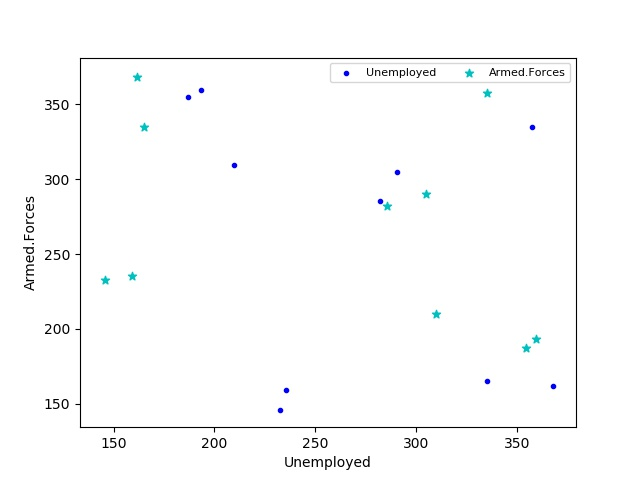
\includegraphics[width=.8\linewidth]{scatter1}
		\caption{created with Matplotlib}
		\label{fig:sfig1}
	\end{subfigure}%
	\begin{subfigure}{.5\textwidth}
		\centering
		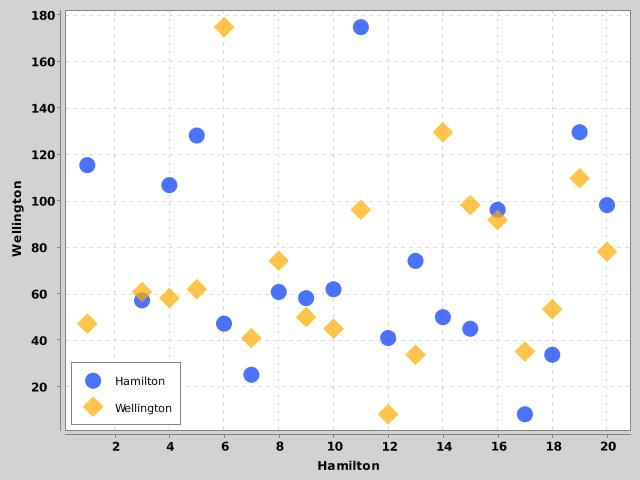
\includegraphics[width=.8\linewidth]{scatter2}
		\caption{created with Jfreechart library}
		\label{fig:sfig2}
	\end{subfigure}
	\caption{Example Scatter plots}
	\label{fig:fig}
\end{figure}


\begin{figure}[!htbp]
	\begin{subfigure}{.5\textwidth}
		\centering
		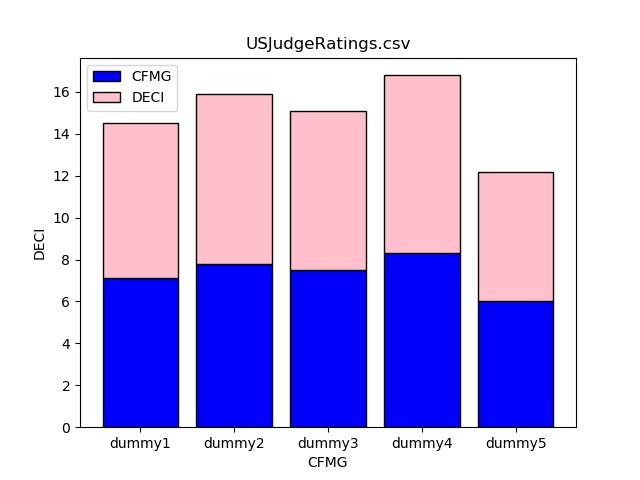
\includegraphics[width=.8\linewidth]{bar1}
		\caption{created in Matlab}
		\label{fig:sfig1}
	\end{subfigure}%
	\begin{subfigure}{.5\textwidth}
		\centering
		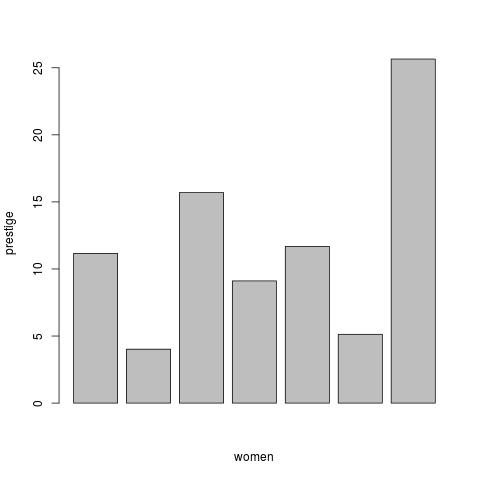
\includegraphics[width=.8\linewidth]{bar2}
		\caption{created in R}
		\label{fig:sfig2}
	\end{subfigure}
	\caption{Example Bar Charts}
	\label{fig:fig}
\end{figure}



\begin{figure}[!htbp]
	\begin{subfigure}{.5\textwidth}
		\centering
		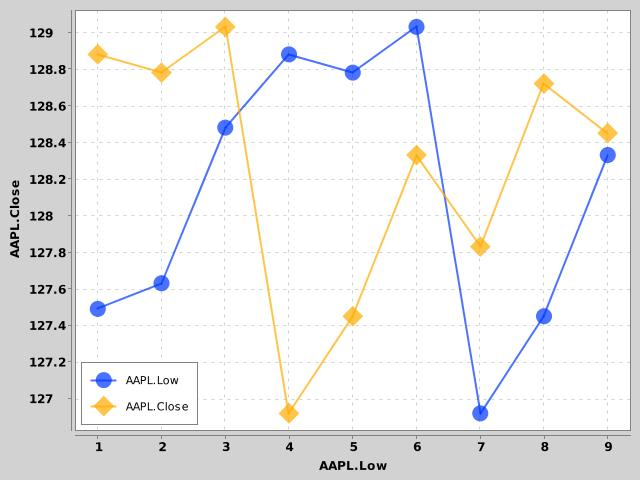
\includegraphics[width=.8\linewidth]{line1}
		\caption{created in Java}
		\label{fig:sfig1}
	\end{subfigure}%
	\begin{subfigure}{.5\textwidth}
		\centering
		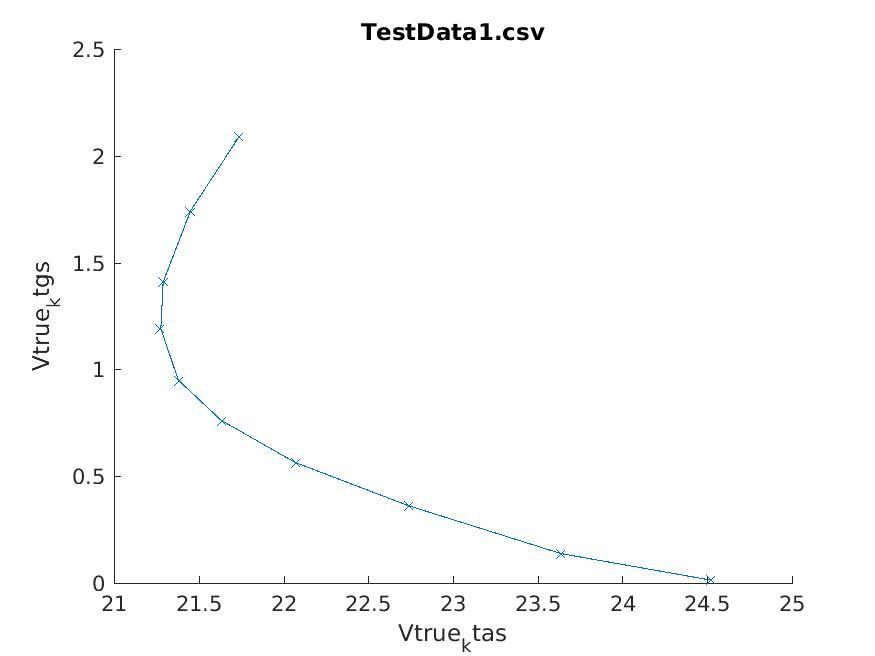
\includegraphics[width=.8\linewidth]{line2}
		\caption{created in Matlab}
		\label{fig:sfig2}
	\end{subfigure}
	\caption{Example Line Charts}
	\label{fig:fig}
\end{figure}



\begin{figure}
	\begin{subfigure}{.5\textwidth}
		\centering
		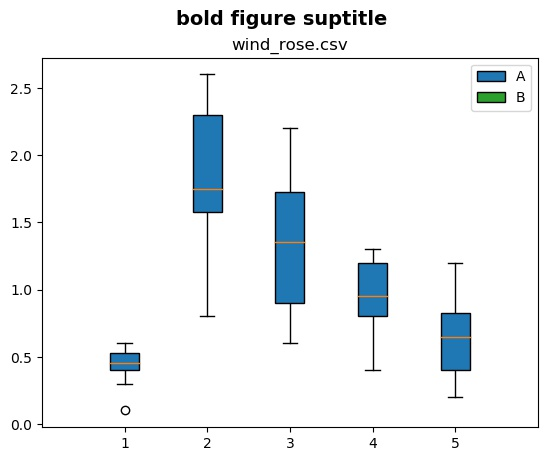
\includegraphics[width=.8\linewidth]{box1}
		\caption{created in python}
		\label{fig:sfig1}
	\end{subfigure}%
	\begin{subfigure}{.5\textwidth}
		\centering
		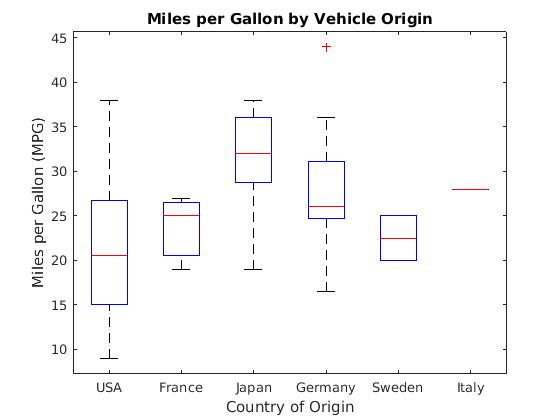
\includegraphics[width=.8\linewidth]{box2}
		\caption{created in Matlab}
		\label{fig:sfig2}
	\end{subfigure}
	\caption{Example Box Plots}
	\label{fig:fig}
\end{figure}


\bibliographystyle{unsrt}
\bibliography{sample}

\end{document}=====